% This is LLNCS.DOC the documentation file of
% the LaTeX2e class from Springer-Verlag
% for Lecture Notes in Computer Science, version 2.4
\documentclass{llncs}
\usepackage{llncsdoc}
\usepackage{graphicx}
\usepackage{amssymb}
\usepackage[table]{xcolor}
\usepackage{listings}

\usepackage{url}
\urldef{\mailwhajwp}\path|{xxx,yyy,zzz}@mini.pw.edu.pl|
\newcommand{\keywords}[1]{\par\addvspace\baselineskip
\noindent\keywordname\enspace\ignorespaces#1}
%
\begin{document}


\title{Title}
\author{xxx$^{1}$
\and yyy$^1$
\and zzz$^{1}$
}

\authorrunning{xxx}
\institute{$^1$Faculty of Mathematics and Information Science, Warsaw University of Technology\\ul. Koszykowa 75, 00-662 Warsaw, Poland\\
%$^2$Department of Electrical \& Computer Engineering, University of Alberta, \\Edmonton T6R 2G7 AB Canada\\
\mailwhajwp
}

\titlerunning{xxxxx yyyyyy zzzzzz}
\maketitle

\pagestyle{empty}  % no page numbers, no running headers

\begin{abstract}
In the article we present
\end{abstract}


%-------------------------------------------------------------------
%-------------------------------------------------------------------
%-------------------------------------------------------------------

\section{Introduction}
  \label{sec:Introduction}

%difference between native and foreign

%why this problem is important

%objectives; what is the contribution of this paper

%novelty elements

%The paper is structured as follows. Section \ref{sec:Literature Review} presents the background knowledge on foreign elements detection present in the literature. Section \ref{sec:preliminaries}


%-------------------------------------------------------------------
%-------------------------------------------------------------------
%-------------------------------------------------------------------
\section{Literature Review}
  \label{sec:Literature Review}

%here on 1- outlier detection, 2 - novelty classification, 3 - foreign elements rejection



%-------------------------------------------------------------------
%-------------------------------------------------------------------
%-------------------------------------------------------------------
\section{Preliminaries}
  \label{sec:preliminaries}

%the task of classification is ...

%...

%-------------------------------------------------------------------
%-------------------------------------------------------------------
\subsection{Ellipsoids for Foreign Elements Rejection}

%description of the idea of geometrical rejection 
%issues: location, size, parameters of those figures

% Links used in this description
% Link: http://geomalgorithms.com/a08-_containers.html
% http://people.orie.cornell.edu/miketodd/TYKhach.pdf
In computational geometry, the smallest enclosing box problem is that of finding the oriented minimum bounding box enclosing a set of points. In many cases there's a need for computing convex hull of set of points and testing inclusions of other points in the same space. This can become very complex problem especially in higher dimensions, so more often an approximation of the hull is used. This helps to reduce time needed for computations, since most of the methods have lower construction and inclusion-testing complexities. Some of such approaches include using figures like hypercubes, diamonds, balls or ellipsoids to successfully enclose given set of points.

When comparing highlights and drawbacks of each method, from computational complexity, ease of testing point inclusion and algorithm implementation point of view, ellipsoids seem very reasonable to choose. Constructed ellipsoid is superior to the minimal cuboid in many ways. It is unique, better approximation of the object it contains and if $E(S)$ is the bounding ellipsoid for a point set $S$ with convex hull $C(S)$ in dimension \textit{d}, then:
\[ \frac{1}{d}E(S) \subseteq C(S) \subseteq E(S) \]
where scaling is with respect to the center of $E(S)$.

%in our experiments we select ellipsoids

%-------------------------------------------------------------------
\subsubsection{MVEE}
%description of MVEE algorithm
% Links used:
% http://citeseerx.ist.psu.edu/viewdoc/download;jsessionid=3A12C2006473A250D78C45B99B0BB3FA?doi=10.1.1.116.7691&rep=rep1&type=pdf
% http://www.mathworks.com/matlabcentral/fileexchange/9542-minimum-volume-enclosing-ellipsoid/content/MinVolEllipse.m
% http://stackoverflow.com/questions/1768197/bounding-ellipse/1768440#1768440
% http://stackoverflow.com/questions/14016898/port-matlab-bounding-ellipsoid-code-to-python

problem is solved by several known algorithms that can be categorized as first-order, second-order interior-point or combination of the two. For small dimensions \textit{d}, the MVEE problem can be solved in \textit{O($d^{O(d)}$m)} operations using randomized or determistic algorithms\cite{MVEEMichaelTodd2005}. In this paper the algorithm based on Khachiyan solution is used.

\noindent An ellipsoid in center form is given by \[ E = \{x \in \mathbb{R}^{n} | (x - c)^{T}A(x-c) \le 1\} \] where $c \in \mathbb{R}^{n}$ is the center of the ellipse E and $ A \in \mathbb{S}^{n}_{++}$ Points lying inside the ellipse satisfy \[ (x_{i} - c)^{T}A(x_{i} - c) \le 1 \]

\noindent The pseudocode for the MVEE algorithm used in this paper is as follows:
\begin{lstlisting}
while err > tolerance
	X = Q * diag(u) * Q'
	M = diag(Q' * inv(X) * Q)
	[maximum j] = max(M)
	step_size = (maximum - d -1)/((d+1)*(maximum-1))
	new_u = (1 - step_size)*u
	new_u(j) = new_u(j) + step_size
	count = count + 1
	err = norm(new_u - u)
	u = new_u
end
\end{lstlisting}

%-------------------------------------------------------------------
%-------------------------------------------------------------------
\subsection{Native Elements Classification}


%now description of those particular classifiers that we use: SVMs, KNNs, ...
%-------------------------------------------------------------------
\subsubsection{Support Vector Machines}
%-------------------------------------------------------------------
% Used links:
% http://scikit-learn.org/stable/modules/svm.html#svm-kernels
are a set of supervised learning methods used for classification, regression and outliers detection. They are effective in high dimensional spaces, memory efficient and quite versatile with many kernel functions that can be specified for the decision function. Although in some cases, where number of features is much greater than the number of samples, this method can give poor results, and is not cost-efficient when calculating probability estimates, it is well suited for problem presented in this paper. Given a set of training examples, each marked for belonging to one of two categories, an SVM training algorithm builds a model that assigns new examples into one category or the other. For multi-class classification "one-against-one" approach is used. For \textit{n} classes \textit{n} * (\textit{n} - 1) / 2 classifiers are constructed, each trains data from two different classes. The order for classes 0 to \textit{n} is "0 vs 1", "0 vs 2", \dots "0 vs \textit{n}", "1 vs 2", \dots "\textit{n} - 1 vs \textit{n}".

\subsubsection{Random Forests}
%-------------------------------------------------------------------
method is based on classification trees, which are used to predict membership of objects in the classes.
For vector of independent variables representing one object they calculate the value of the class the object belongs to by dividing value space into two or more subspaces. More precisely, an input data is entered at the top of the tree and as it traverses down the tree the data gets bucketed into smaller and smaller sets.
The main principle behind the Random Forest method is that a group of "weak learners" can come together to form a "strong learner". 
After a large number of trees is generated, they vote for the most popular class.
We call these procedures random forests.
\subsubsection{K-Nearest Neighbors}

%-------------------------------------------------------------------
%-------------------------------------------------------------------
\subsection{Quality Evaluation}

%measures for quality evaluation: precision, recall, ...
\begin{itemize}
\item CC  (Correctly Classified) - the number of correctly classified patterns, i.e. native patterns classified as native ones with the correct class, % and foreign patterns classified as foreign ones,
\item TP  (True Positives) - the number of native patterns classified as native (no matter, into which native class),
\item FN  (False Negatives) - the number of native patterns incorrectly classified as foreign,
\item FP  (False Positives) - the number of foreign patterns incorrectly classified as native,
\item TN  (True Negatives) - the number of foreign patterns correctly classified as foreign.
\end{itemize}



\begin{eqnarray}
            \textnormal{Accuracy} &\!\!=\!\!& \frac{\textnormal{TP+TN}}{\textnormal{TP+FN+FP+TN}}\nonumber\\\nonumber\\
     \textnormal{Strict Accuracy} &\!\!=\!\!& \frac{\textnormal{CC+TN}}{\textnormal{TP+FN+FP+TN}}\nonumber\\\nonumber\\
    \textnormal{Native Precision} &\!\!=\!\!& \frac{\textnormal{TP}}{\textnormal{TP+FP}}\nonumber\\\nonumber\\
  \textnormal{Native Sensitivity} &\!\!=\!\!& \frac{\textnormal{TP}}{\textnormal{TP+FN}}\nonumber\\\nonumber\\
  \textnormal{Strict Native Sensitivity} &\!\!=\!\!& \frac{\textnormal{CC}}{\textnormal{TP+FN}}\nonumber\\\nonumber\\
          \textnormal{Fine Accuracy} &\!\!=\!\!& \frac{\textnormal{CC}}{\textnormal{TP}}\nonumber\\\nonumber\\
   \textnormal{Foreign Precision} &\!\!=\!\!& \frac{\textnormal{TN}}{\textnormal{TN+FN}}\nonumber\\\nonumber\\
 \textnormal{Foreign Sensitivity} &\!\!=\!\!& \frac{\textnormal{TN}}{\textnormal{TN+FP}}\nonumber\\\nonumber\\
          \textnormal{F--measure} &\!\!=\!\!& 2\cdot\frac{\textnormal{Precision}\cdot\textnormal{Sensitivity}} {\textnormal{Precision}+\textnormal{Sensitivity}}\nonumber\\\nonumber
\end{eqnarray}


\begin{itemize}
  \item \emph{Strict Accuracy} is the absolute measure of the classifier's performance. It is the ratio of the number of all \emph{correctly} classified patterns, i.e. native patterns classified to their respective classes and rejected foreign ones to the number of all patterns being processed.
  \item \emph{Accuracy} is a characteristic derived from strict accuracy by ignoring the need to classify native patterns to their respective classes; in other words, it is sufficient to correctly identify whether a~pattern is native or foreign one. This measure describes the ability to distinguish between native and foreign patterns.
  \item \emph{Native Precision} is the ratio of the number of not rejected native patterns to the number of all not rejected patterns (i.e. all not rejected native and foreign ones). Native Precision evaluates the ability of the classifier to distinguish native patterns from foreign ones. The higher the value of this measure, the better ability to distinguish foreign elements from native ones. Native Precision does not evaluate how effective identification of native elements is.
  \item \emph{Native Sensitivity} is the ratio of the number of not rejected native patterns to all native ones. This measure evaluates the ability of the classifier to identify native elements. The higher the value of Native Sensitivity, the more effective identification of native elements. Unlike the Native Precision, this measure does not evaluate the effectiveness of separation between native and foreign elements.
  \item \emph{Strict Native Sensitivity} takes only correctly classified native patterns and does not consider native patterns, which are not rejected and assigned to incorrect classes, unlike \emph{Native Sensitivity}, where all not rejected native patterns are taken into account.
  \item \emph{Fine Accuracy} is the ratio of the number of native patterns classified to correct classes, i.e. assigned to their respective classes, to the number of all native patterns not rejected. This measure conveys how precise is correct classification of not rejected patterns.
  \item \emph{Foreign Precision} corresponds to Native Precision.
  \item \emph{Foreign Sensitivity} corresponds to Native Sensitivity.
  \item  Precision and Sensitivity are complementary and there exists yet another characteristic that combines them: the \textit{F--measure}. It is there to express the balance between precision and sensitivity since these two measures affect each other. Increasing sensitivity can cause a~drop in precision since, along with correctly classified elements, there might be more incorrectly classified,
\end{itemize}

%-------------------------------------------------------------------
%-------------------------------------------------------------------
%-------------------------------------------------------------------
\section{Experiments}
  \label{sec:Experiments}

%-------------------------------------------------------------------
%-------------------------------------------------------------------
\subsection{Presentation of Datasets}

Figure \ref{fig:nativeforeignpatterns} presents native and foreign patterns ...

\begin{figure}[!t]
  \centering
  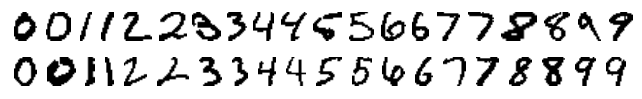
\includegraphics[width=0.49\textwidth]{_Figures/native}
  \caption{...}
\label{fig:nativeforeignpatterns}
\end{figure}


%-------------------------------------------------------------------
%-------------------------------------------------------------------
\subsection{Impact on Classification}

%ideally rejection improves classification by rejecting those element that would have been incorrectly classified

\begin{table*}[t]
\centering
\caption{Results for classification with rejection on train and test sets of native patterns in comparison with classification results without rejection mechanism. RF - results for random forest, SVM - results for Support Vector Machines, ....}
\vspace{3pt}
\setlength{\tabcolsep}{6pt}
\renewcommand{\arraystretch}{1}
\begin{tabular}{|r||cccc|cccc|}
\hline
& \multicolumn{4}{c|}{no rejection} & \multicolumn{4}{c|}{with rejection}  \\
\hline
  Basic Classifier & RF & SVM & KNN &  & RF & SVM & KNN &  \\
\hline
  Data Set & \multicolumn{8}{c|}{Native Patterns, Train Set} \\
\hline
Fine Accuracy                & $$ & $$ & $$ & $$ & $$ & $$ & $$ & $$ \\
Strict Native Sensitivity    & $$ & $$ & $$ & $$ & $$ & $$ & $$ & $$ \\
Native Sensitivity           & $$ & $$ & $$ & $$ & $$ & $$ & $$ & $$ \\
\hline
  Data Set & \multicolumn{8}{c|}{Native Patterns, Test Set} \\
\hline
Fine Accuracy                & $$ & $$ & $$ & $$ & $$ & $$ & $$ & $$ \\
Strict Native Sensitivity & $$ & $$ & $$ & $$ & $$ & $$ & $$ & $$ \\
Native Sensitivity        & $$ & $$ & $-$ & $-$ & $$ & $$ & $-$ & $-$ \\
\hline
\end{tabular}
\vspace{12pt}
\label{tab:NativeNoForeign}
\end{table*}


%-------------------------------------------------------------------
%-------------------------------------------------------------------
\subsection{Rejection Quality}

\begin{table*}[!htb]
\centering
\caption{Results of classification with rejection on the set of native patterns supplemented with different sets of semi-synthetic  foreign patterns....}
\vspace{3pt}
\setlength{\tabcolsep}{4pt}
\renewcommand{\arraystretch}{1}
\begin{tabular}{||r||ccccc||ccccc||}
\hline
  Basic Classifier & RF & SVM & KNN &  &  &  RF & SVM & KNN &  &  \\
\hline
  Data Set & \multicolumn{5}{c||}{ xxx } & \multicolumn{5}{c|}{ x x } \\
\hline
\hline
Strict Accuracy     &&&&&&&&&& \\
Accuracy            &&&&&&&&&& \\
Native Precision    &&&&&&&&&&  \\
Native Sensitivity  &&&&&&&&&&  \\
Foreign Precision   &&&&&&&&&&  \\
Foreign Sensitivity &&&&&&&&&&  \\
Native F-measure    &&&&&&&&&& \\
Foreign F-measure   &&&&&&&&&&  \\
\hline
\hline
  Data Set & \multicolumn{5}{c||}{ yyy } & \multicolumn{5}{c|}{ zzz } \\
\hline
\hline
Strict Accuracy     &&&&&&&&&&  \\
Accuracy            &&&&&&&&&& \\
Native Precision    &&&&&&&&&&  \\
Native Sensitivity  &&&&&&&&&&  \\
Foreign Precision   &&&&&&&&&&  \\
Foreign Sensitivity &&&&&&&&&& \\
Native F-measure    &&&&&&&&&&  \\
Foreign F-measure   &&&&&&&&&&  \\
   \hline
\end{tabular}
\vspace{12pt}
\label{tab:rejection_results}
\end{table*}


%-------------------------------------------------------------------
%-------------------------------------------------------------------
%-------------------------------------------------------------------
\section{Conclusion}
  \label{Conclusion}

Proposed ...

In future ...

%-------------------------------------------------------------------
%-------------------------------------------------------------------
%-------------------------------------------------------------------

\section*{Acknowledgment}

\noindent The research is partially supported by the .....

%-------------------------------------------------------------------
%-------------------------------------------------------------------
%-------------------------------------------------------------------
\begin{thebibliography}{1}

\bibitem{HempstalkFrankWitten2008}
Hempstalk, K., Frank, E., Witten, I., \emph{One-class classification by combining density and class probability estimation}, Machine Learning and Knowl. Disc. in Databases, pp. 505-519, 2008.

\bibitem{MVEEMichaelTodd2005}
Michael J. Todd, E.Alper Yildirim, \emph{On Khachiyan's Algorithm for the Computation of Minimum Volume Enclosing Ellipsoids}, September 30, 2005, article link: http://people.orie.cornell.edu/miketodd/TYKhach.pdf


\end{thebibliography}



\end{document}
